\chapter{Výsledky simulace}

\section{Gzebo svět}

Na základě diplomové práce studenta bc. Miloše Cihlářa 

\section{Let po waypointech}

Funkčnost simulace jsme demonstrovali na robotické misi jejímž cílem byl let dronu po waypointech. Pro tento účel jsme implementovali dvě alternativy, a to řízení dronu na lokální, a globální waypointy. V obou případech jsou data o trajektorii letu známá před misí. Tyto data se načítají z \texttt{.yaml} souboru jako ROS 2 parametry, takže je možné je měnit bez kompilace celého zdrojového kódu mise. 

\subsection{Let podle lokálních waypointů}

Zprávy typu \texttt{geometry\_msgs::msg::PoseStamped} jsou z nadřazeného uzlu publikovány do ROS 2 témy (\textit{topic}) \texttt{/mavros/setpoint\_position/local} s frekvencí 10 Hz (pro aktivitu \textit{offboard} letového režimu musí být zprávy posílány s frekvencí > 2 Hz).

\subsection{Let podle globálních waypointů}

Zprávy typu \texttt{geographic\_msgs::msg::GeoPoseStamped} jsou z nadřazeného uzlu publikovány do ROS 2 témy (\textit{topic}) \texttt{/mavros/setpoint\_position/global} s frekvencí 10 Hz.

\section{Let podle setpointů rychlosti}

Další robotická mise, na které jsme otestovali funkčnost simulace je založená na řízení dronu podle lineární rychlosti v osách X, Y, Z a rychlosti rotace kolem osy Z. 

Řízení tohoto typu je vhodné v případě, že regulační smyčka v PX4 (obrázek \ref{fig:PX4controller}) nepostačuje našim požadavkům na regulaci a tudíž musíme implementovat vlastní, komplexnější řídící strukturu. Obrázek \ref{fig:PX4controller} zobrazuje, že při řízení dronu pomocí setpointů rychlosti vynecháme PX4 poziční regulátor\footnote{Poziční regulátor V PX4 je složený z P složky a saturace} z řídící struktury.

Další možností, kterou jsme neimplementovali je řízení dronu pomocí setpointů zrychlení. Tímto krokem by jsme vynechali taky rychlostní regulátor\footnote{Rychlostní regulátor V PX4 je složený z PID složky a saturace} a měli by jsme volnou ruku při implementaci komplexnějších řídících struktur.

\begin{figure}[!ht]
  \begin{center}
    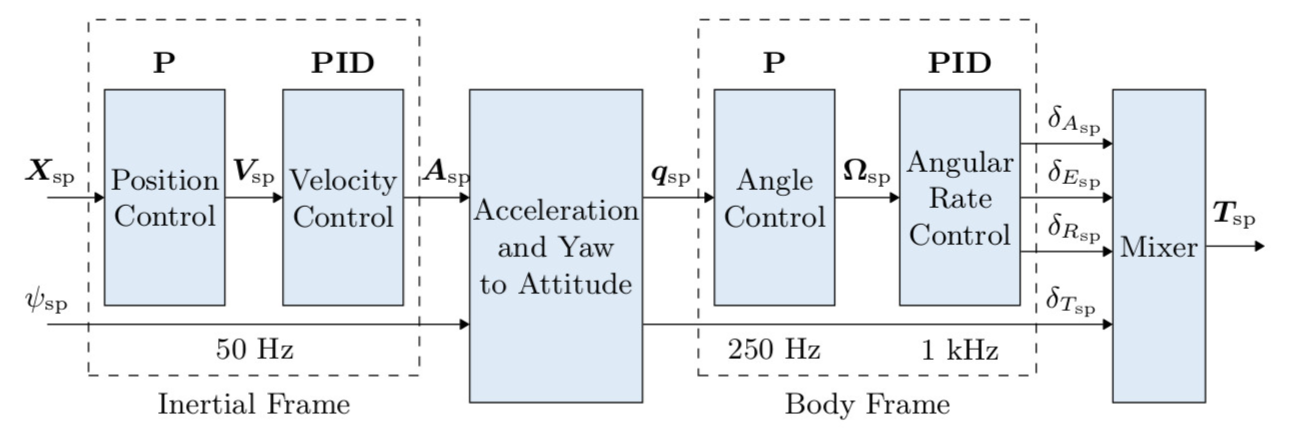
\includegraphics[scale=0.44]{obrazky/PX4CONTROLLER}
  \end{center}
  \caption[Řídící struktura systému PX4]{Řídící struktura systému PX4. \cite{PX4docs}}
  \label{fig:PX4controller}
\end{figure}

Zprávy typu \texttt{geometry\_msgs::msg::TwistStamped} jsou z nadřazeného uzlu publikovány do ROS 2 témy (\textit{topic}) \texttt{/mavros/setpoint\_velocity/cmd\_vel} s frekvencí 10 Hz.

\section{Mise pro sledování dynamického objektu}

Funkčnost simulace jsme také demonstrovali na složitější robotické misi jejímž cílem bylo sledování dynamického objektu. 

Pro tuto úlohu jsme využili data z měření radiace pomocí všesměrového radiačního detektoru, který byl umístěný na pozemním robotu. Robot pomocí částicového filtru (\textit{particle filter}) estimoval pozici radioaktivního zářiče a na základě této estimace se k zdroju radiace přibližoval.

Data z měření jsme měli k dispozici jako \texttt{rosbag} soubor\footnote{Rosbag soubor slouží na zálohu dat v podobě ROS 2 témat (\textit{topic})}, který obsahuje zprávy typu \texttt{geographic\_msgs::msg::GeoPoseStamped} a publiku je do ROS 2 tématu \texttt{/estimated\_source\_location}. Tyto zprávy obsahují globální souřadnice estimovaného zdroje radiace podle standardu WGS 84. Dron se v průběhu celé mise pohybuje v konstantní výšce, která de definovatelná uživatelem pomocí ROS 2 parametru.

\begin{figure}[!ht]
  \begin{center}
    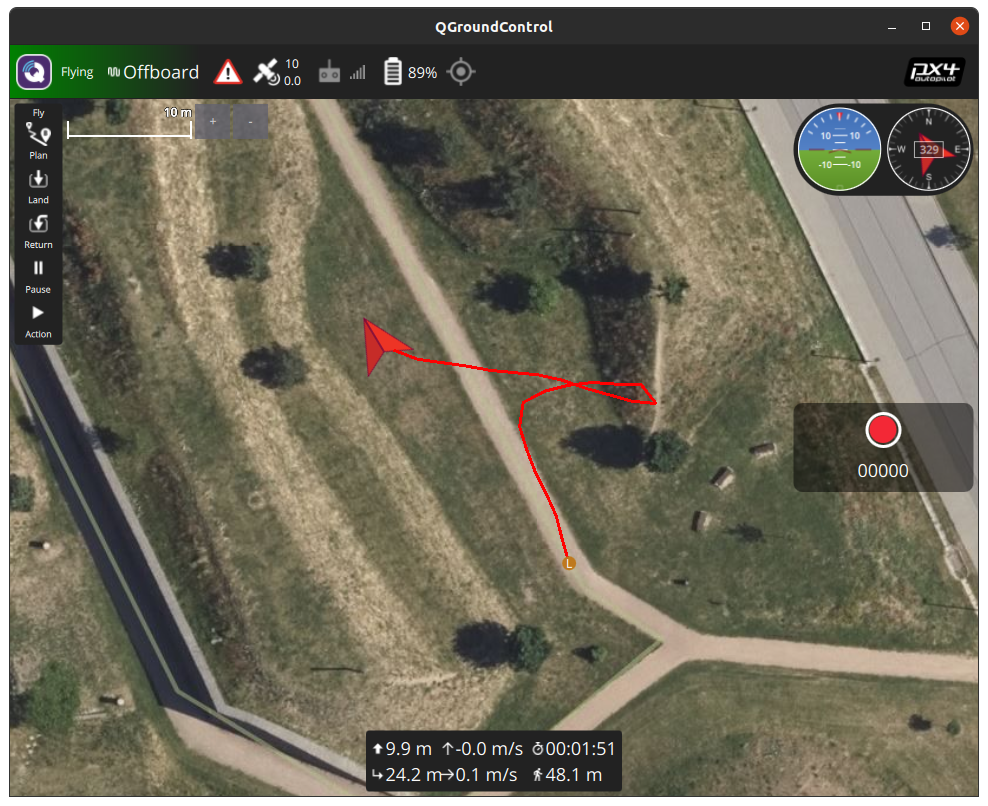
\includegraphics[scale=0.35]{obrazky/MISESL1}
  \end{center}
  \caption[Software QGroundControl s dronem v \textit{offboard flight mode}]{Software QGroundControl s dronem v \textit{offboard flight mode}.}
  \label{fig:SIM3QGC}
\end{figure}

\begin{figure}[!ht]
  \begin{center}
    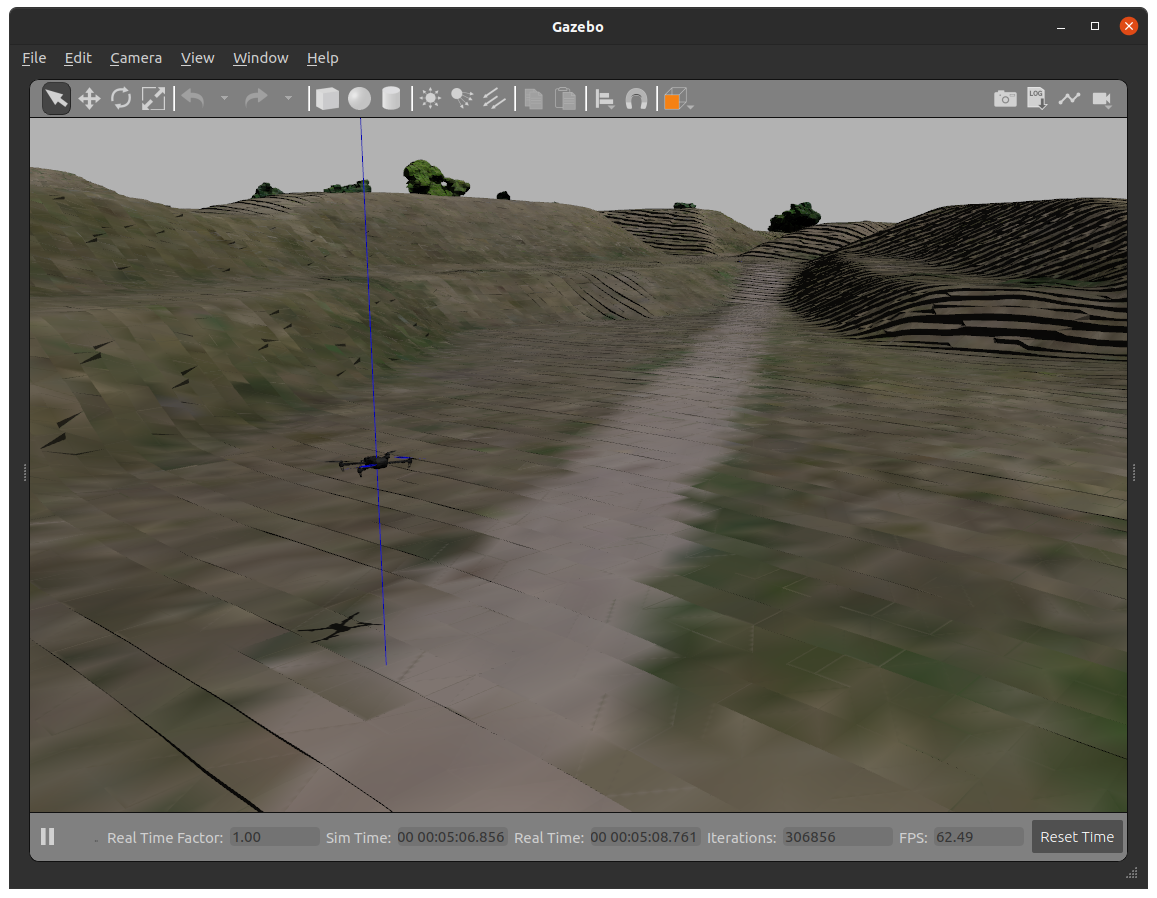
\includegraphics[scale=0.3]{obrazky/GAZSIMPLE.png}
  \end{center}
  \caption[Software QGroundControl s dronem v \textit{offboard flight mode}]{Software QGroundControl s dronem v \textit{offboard flight mode}.}
  \label{fig:SIM3GAZ}
\end{figure}


\section{Simulace mise s více drony}

DOKONČIŤ

\begin{figure}[!ht]
  \begin{center}
    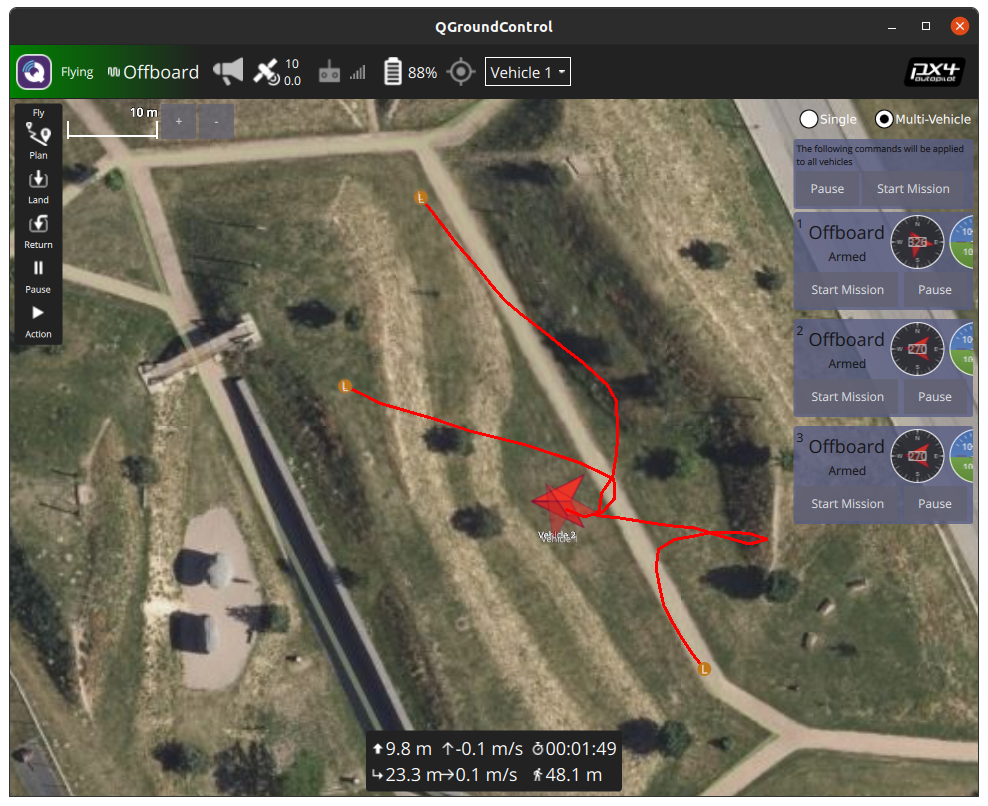
\includegraphics[scale=0.33]{obrazky/QGMULTIPLE.png}
  \end{center}
  \caption[Software QGroundControl s dronem v \textit{offboard flight mode}]{Software QGroundControl s dronem v \textit{offboard flight mode}.}
  \label{fig:SIM3MULQG}
\end{figure}

\begin{figure}[!ht]
  \begin{center}
    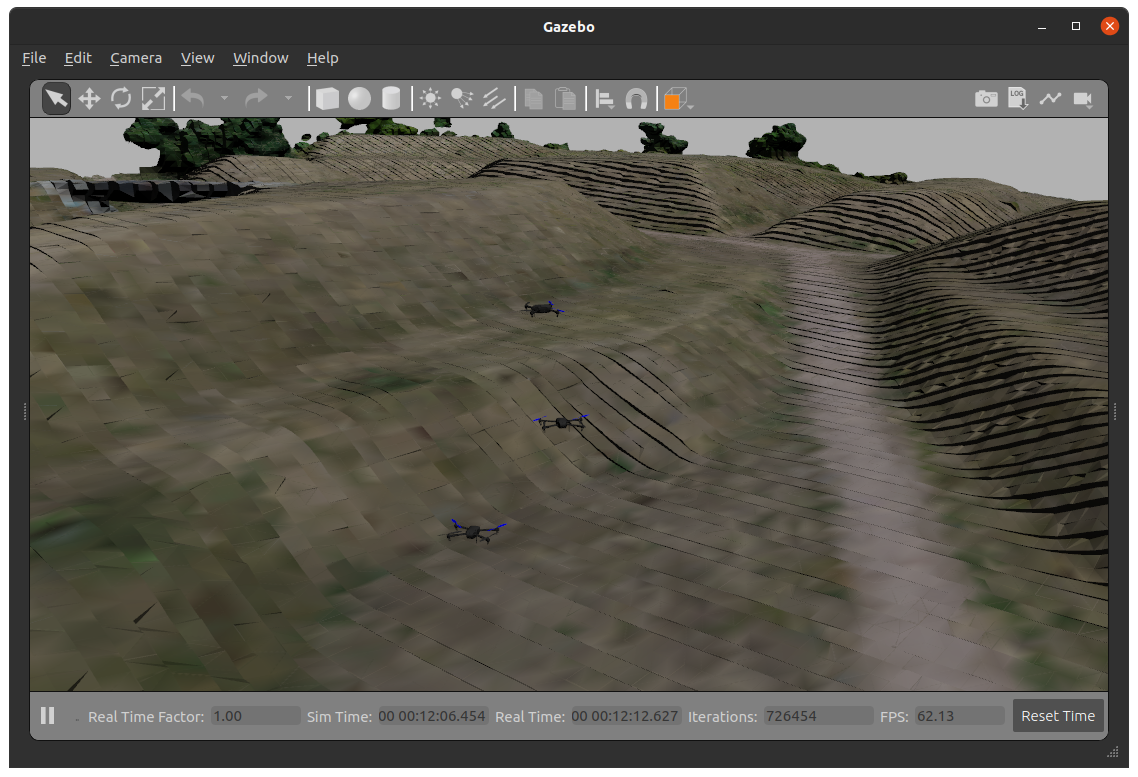
\includegraphics[scale=0.32]{obrazky/GAZMULTIPLE.png}
  \end{center}
  \caption[Software QGroundControl s dronem v \textit{offboard flight mode}]{Software QGroundControl s dronem v \textit{offboard flight mode}.}
  \label{fig:SIM3MULGAZ}
\end{figure}
